\documentclass[10pt,twocolumn,letterpaper]{article}

\usepackage{icb}
\usepackage{times}
\usepackage{epsfig}
\usepackage{graphicx}
\usepackage{amsmath}
\usepackage{amssymb}
\usepackage{eso-pic}

% Include other packages here, before hyperref.

% If you comment hyperref and then uncomment it, you should delete
% egpaper.aux before re-running latex.  (Or just hit 'q' on the first latex
% run, let it finish, and you should be clear).
%\usepackage[pagebackref=true,breaklinks=true,letterpaper=true,colorlinks,bookmarks=false]{hyperref}

\icbfinalcopy % *** Uncomment this line for the final submission

\def\icbPaperID{****} % *** Enter the IJCB Paper ID here
\def\httilde{\mbox{\tt\raisebox{-.5ex}{\symbol{126}}}}

% Pages are numbered in submission mode, and unnumbered in camera-ready
\ificbfinal\pagestyle{empty}\fi
\begin{document}

%%%%%%%%% TITLE
\title{Investigation of muscular architecture in ultrasound images}

\author{Thomas Bergmueller, Martin Schnoell\\
Medical Imaging LAB\\
Master program: Applied Image and Signal Processing\\
Fachhochschule Salzburg\\
%Institution1 address\\
{\tt\small tbergmueller.aise-m2013@fh-salzburg.ac.at, mschnoell.aise-m2013@fh-salzburg.ac.at}
% For a paper whose authors are all at the same institution,
% omit the following lines up until the closing ``}''.
% Additional authors and addresses can be added with ``\and'',
% just like the second author.
% To save space, use either the email address or home page, not both
%\and
%Second Author\\
%Institution2\\
%First line of institution2 address\\
%{\tt\small secondauthor@i2.org}
}

\maketitle
\thispagestyle{empty}

%%%%%%%%% ABSTRACT
\begin{abstract}
   The ABSTRACT is to be in fully-justified italicized text, at the top
   of the left-hand column, below the author and affiliation
   information. Use the word ``Abstract'' as the title, in 12-point
   Times, boldface type, centered relative to the column, initially
   capitalized. The abstract is to be in 10-point, single-spaced type.
   Leave two blank lines after the Abstract, then begin the main text.
   Look at previous ICB abstracts to get a feel for style and length.
\end{abstract}

%%%%%%%%% BODY TEXT

\section{Introduction}
The main goal of this project was to write an algorithm which automatically calculates the angle between the aponeurosis and the muscle fibers of the Vastus Lateralis which is the muscle on the thigh right over the knee. This angle correlates with the constitution of the muscle.
For this project we used ultrasound images.  
Figure \ref{fig:VastusLateralis} shows the location of the Vastus Lateralis and an example ultrasound image in which both aponeuroses (lower and upper one) as well as the desired angle is drawn (dashed line).

\begin{figure}
	\begin{center}		
		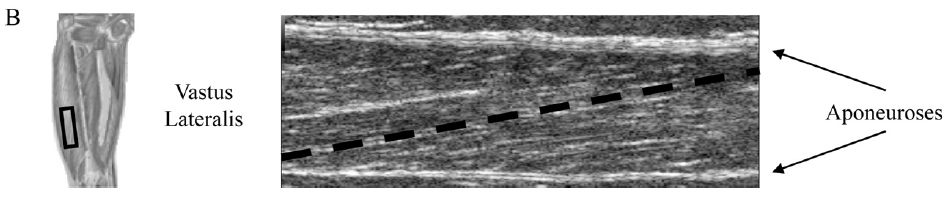
\includegraphics[width=1\linewidth]{img/VastusLateralis}
	\end{center}
	\caption{Vastus Lateralis (left) and an example ultrasound image in which both aponeuroses (lower and upper one) as well as the desired angle is drawn (dashed line). \cite{NCronin13a}}
	\label{fig:VastusLateralis}
	
\end{figure}

Usually, this angle is calculated manually, by fitting lines to an ultrasound image on the computer and then calculate the angle by hand.

The available groundtruth consists of 22 ultrasound images of the Vastus Lateralis from 12 different patients.
Figure \ref{fig:exImage} shows one original image of the dataset.

\begin{figure}
	\begin{center}		
		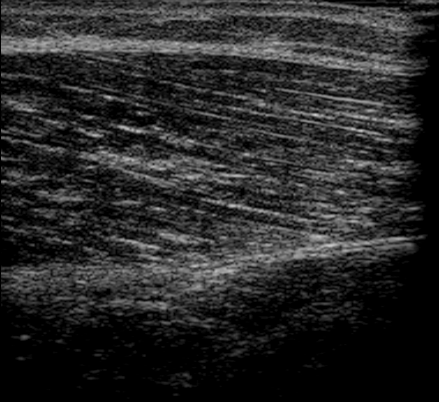
\includegraphics[width=1\linewidth]{img/COLLINI_1_cropped}
	\end{center}
	\caption{One original image of the dataset.}
	\label{fig:exImage}
	
\end{figure}

For every image two or three different measurements of the angle exist, which partly vary significantly. For example, is the biggest difference of two measurements for the same image (!) 5.7 degree (DOPPLER\_1.bmp). In the most cases, however, the single measurements are in the range of +/- 1.5 to the mean.
For our implementation we calculated the mean angle of all measurements from one image and took this mean angle as a reference.

\section{Proposed algorithms}
We worked on two different algorithms in order to determine the angle. The first one is the Hough transform, which is a well-known algorithm for detecting lines in an image. The second one is based on template matching. ...Here, one patch is determined and shifted over the images, looking for matches...

\subsection{Hough transform}
The Hough transform is a well-known and established algorithm for detecting lines and other shapes in images. For the implementation, we used MATLAB R2013a and the inbuilt MATLAB function hough.
This are the main steps of our implementation:

\begin{enumerate}
     \item Gamma correction for enhancing the white pixels
     \item Binarization of the image
     \item Hough transform applied directly on the binary image in order to detect the aponeurosis
     \item Canny edge detection on the binary image
     \item Hough transform on the edge image
     \item Finally: Calculate the mean of all valid muscle fibers and then determine the difference between the angle of the aponeurosis and the mean. This results in the final desired angle
\end{enumerate}



\subsection{Template Matching}
...

\section{Comparison of both algorithms}
The average error/distance for all 22 images of both approaches: Hough transform: 2.48 degree. Template matching: 3.06 degree.

Figure \ref{fig:errorPlot} shows the error plot of both algorithms.

\begin{figure}
	\begin{center}		
		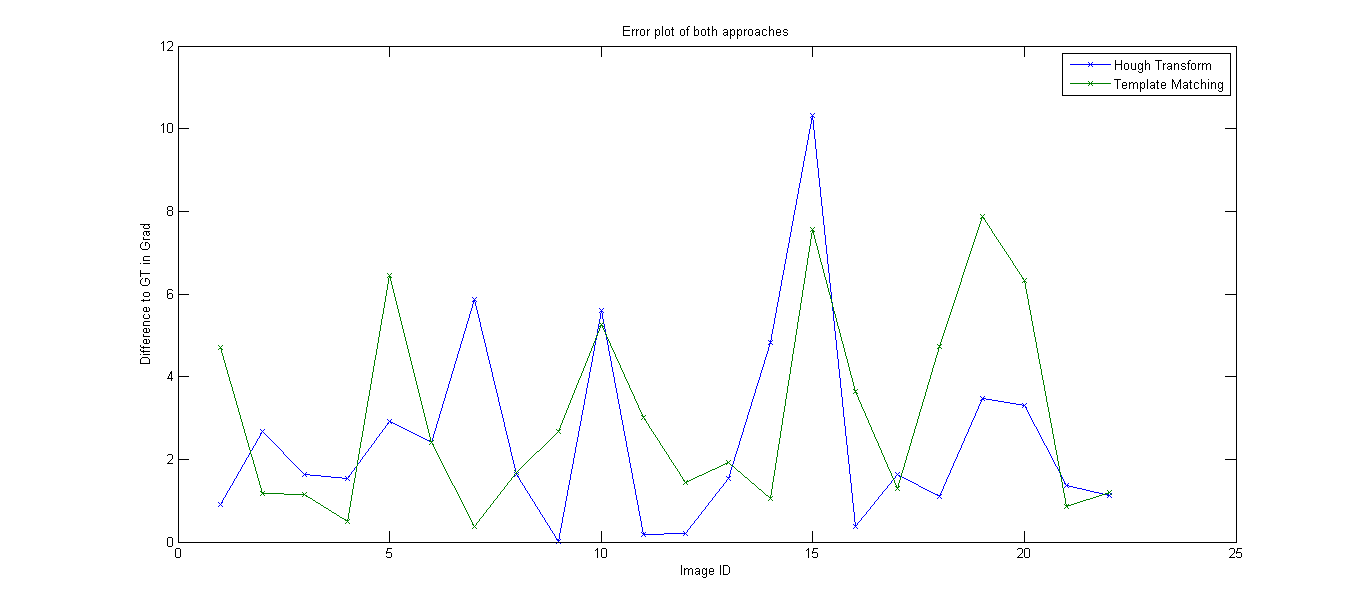
\includegraphics[width=1\linewidth]{img/error_plot}
	\end{center}
	\caption{One original image of the dataset.}
	\label{fig:errorPlot}
	
\end{figure}

\section{Conclusion}
There are images where the automatic angle calculation works well, but there are also images were it doesn't work so well...

{\small
\bibliographystyle{ieee}
\bibliography{egbib}
}

\end{document}
